\section{Optimizing Nonlinear Circuits}
While effective heuristics exist for optimizing linear circuits to reduce the number of required XOR gates, the problem becomes significantly more difficult if variables the straight line program can be multiplied together. As multiplication can usually be regarded as a more expensive operation than addition, we are generally interested in minimizing the number of multiplications required to compute a particular function. In NAND-based CMOS technology, AND/NAND gates are significantly cheaper than XOR gates because the former are used to build the latter. We disregard this detail for the purpose of working on the more general problem of minimizing the required multiplication operations, which is known as the \emph{multiplicative complexity}. In fact, this is the problem that motivated the two-step Boolean logic minimization technique pioneered by Boyar and Peralta \cite{Boyar12-1}. Shannon \cite{Shannon49-1} and Lupanov \cite{Lupanov58-1} showed that \emph{almost all} Boolean functions on $n$ inputs have a Boolean circuit complexity of about $\frac{2^n}{n}$, and Boyar et al. \cite{Boyar00-1} later showed that the common multiplicative complexity is $2^{n/2}$. Of course, these upper bounds do not hold for all Boolean functions, and as such, the problem of optimizing nonlinear circuits (or parts of a circuit) is related to the difficulty of attaining functions with polynomial multiplicative complexity. In this work we assume that the Boolean functions are not symmetric. That is, the output of such functions does not depend solely on the Hamming weight of the input. Given that this is a much more difficult problem to solve than symmetric Boolean functions \cite{Boyar00-1}, the more effective techniques for finding minimal nonlinear circuits have been randomized, heuristic-based searches. In the following section we describe some relevant techniques that have been applied in the context of cryptography and discuss our modifications on multiplicative inversion circuits for $GF(2^4)$.

% \todo[inline]{State the goal as trying to minimize the...}
% \todo[inline]{Discussion of Shannon's Boolean complexity stuff and the upper bounds...}
% \todo[inline]{Overview of peralta's technique and difficulty of the problem}
% \todo[inline]{Discussion of my heuristic varying number of XOR rounds and AND rounds...}

\subsection{Ad-Hoc Heuristics}
Perhaps the most effective heuristic to date for optimizing small nonlinear components of large circuits is the ad-hoc search heuristic developed by Boyar and Peralta \cite{Boyar12-1}. Inspired by techniques from automatic theorem proving, the core of their algorithm tries to construct an equivalent small area and low depth function for a given input function. Boyar and Peralta refer to the input columns of the truth table for a Boolean function $f$ as \emph{known signals}, and the output column of the same truth table as the signal of $f$. Then, for any two known signals $u$ and $v$ for functions $g$ and $h$, the sum $u \oplus v$ (product $u \land v$) is equivalent to the signal of the function $g \oplus h$ ($g \land h$). 

Their ad-hoc optimization algorithm wraps this function construction technique with a randomized search for an optimal function $g$ that is equivalent to the input function $f$ but has a lower multiplicative complexity. The iterations of this search are then divided into XOR and AND rounds, each of which will randomly select a specified number of signal pairs $(u, v)$ from the signal set of a working function $f$ and then compute their sum or product, depending on the type of round. Then, the algorithm checks to see if the resulting function $u \oplus v$ or $u \land v$ is equivalent to the input function $f$, and if so, returns the result as $g$. Otherwise, the new function is added to the set of known signals for the working function and the rounds continue. If at any point the number of AND gates exceeds a given threshold, or if the size of the known signal set exceeds a predefined depth, then the randomized algorithm restarts. 

This general procedure is followed for all input functions $f_1,\dots,f_n$, and in an effort to maximize signal reuse among each of the input functions, all of the signals computed during the XOR and AND rounds of a single function $f_i$ are saved for use optimizing all functions $f_j$, $j > i$. Since the functions that are stored vary depending on the order in the input functions $f_1,\dots,f_n$ are optimized, Boyar and Peralta tried all $n!$ permutations of the input set to find an optimized circuit for the nonlinear inversion circuit for $GF((2^2)^2)$ using the normal bases $[V, V^2]$ and $[W, W^4]$ (see the following chapter for more information). We modified and applied their optimization technique to the other $17$ inversion circuits for $GF((2^2)^2)$. The modifications include the ability to specify the number of gates added per AND/XOR round, as well as two evolving probabilities $p_x$ and $p_a$ that determine whether or not a gate is added in each round.

% We also developed our own heuristic that seeks to find an equivalent circuit for a set of linear
% forms by looking at the entire linear system at once, rather than iteratively trying to 
% construct one individual circuit at a time that reuses signals from previous iterations of 
% the algorithm. Our approach is inspired by the intuition that signals which are shared among
% more XOR and AND operations are preferred to those that are not shared. To maintain the 
% the ``fan-out'' of a particlar signal $u$, i.e. the number of signals that were created 
% using $u$, signals are created, stored, and updated as directed graphs representing where the source 
% vertices represent the input signals and the sink vertex represents the current signal ``value''.

% The algorithm for finding a circuit proceeds with XOR and AND rounds as in Boyar and
% Peralta's technique, with the additional operation of pruning the signal tree after a fixed number of 
% rounds. The pruning operation can apply a variety of heuristics for trimming the size of the tree 
% without removing those signals that have resulted in one of the $m$ output signals. The main strategy
% for removing signals in the tree is to remove the path in the tree that starts at a leaf node
% and has the maximum weight. We experimented with several other heuristics to test the effectiveness 
% of our approach, as shown in Figure \ref{fig:signalTreePrune}.
% \begin{figure}
% \begin{center}
% 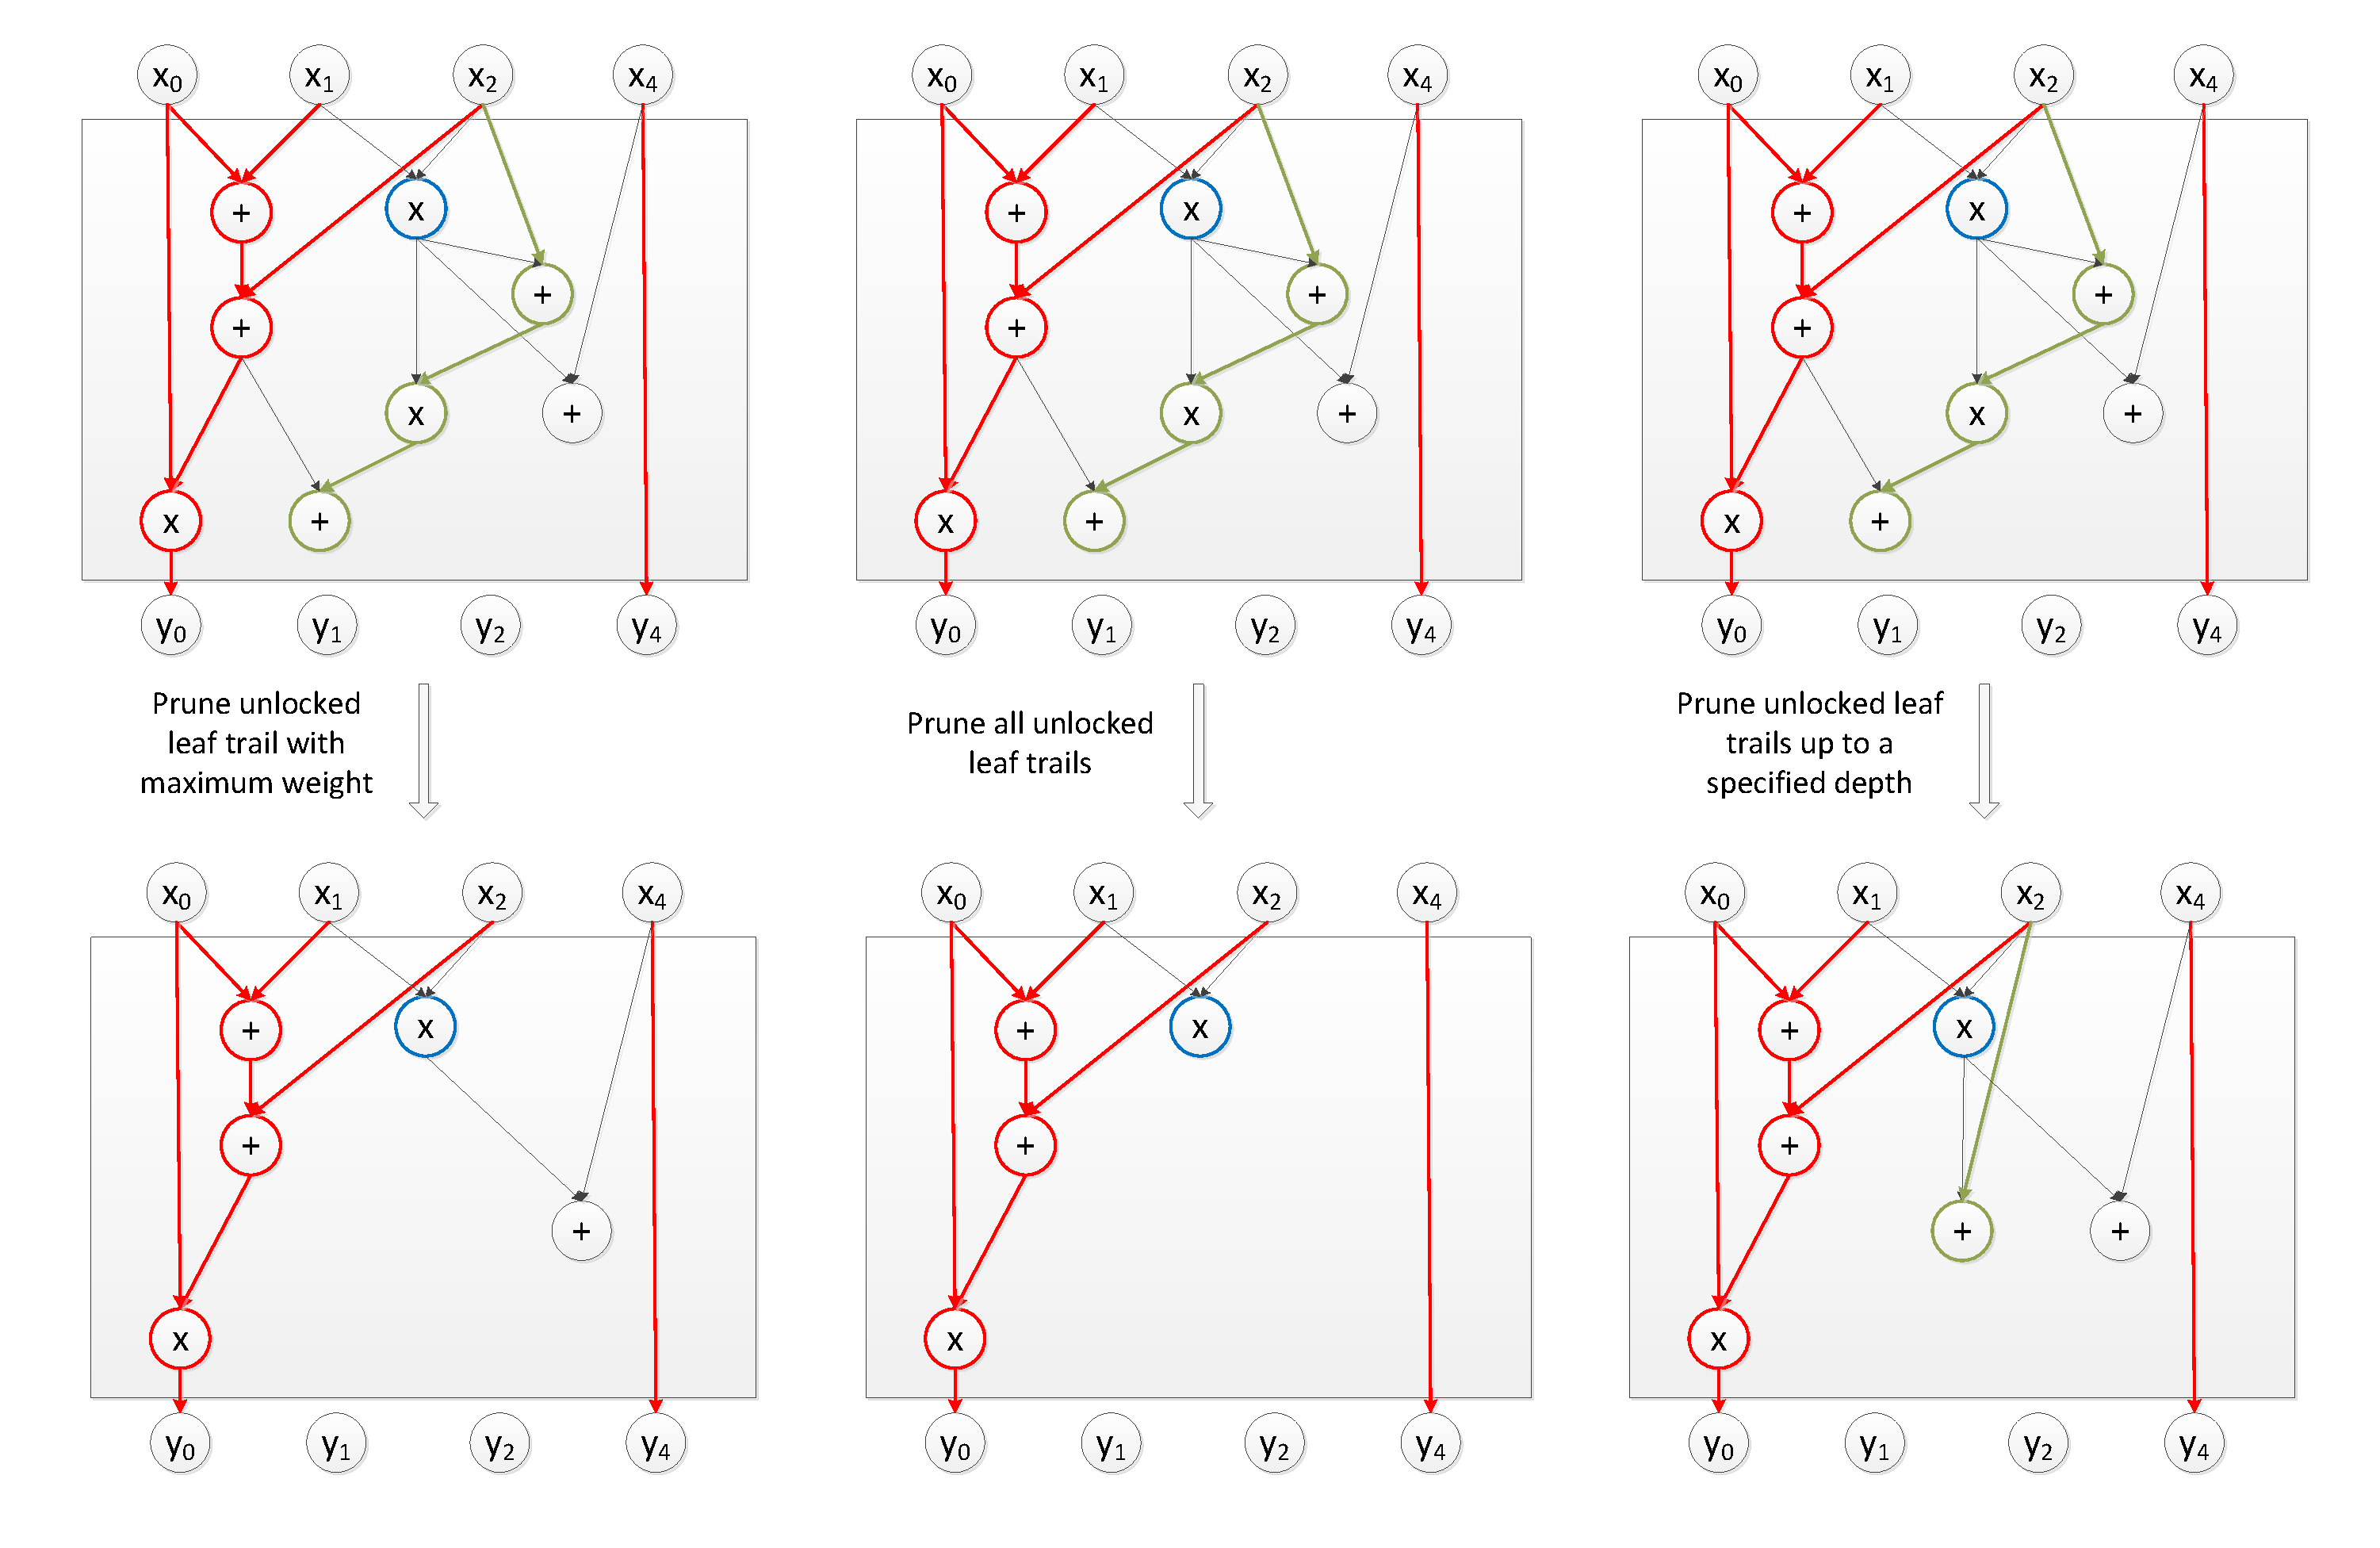
\includegraphics[scale=0.3]{./chapter_optimize/signal_graph.pdf}
% \caption{Visual depiction of several signal tree pruning strategies that were tried during our experiments.}
% \label{fig:signalTreePrune}
% \end{center}
% \end{figure}

\subsection{An Application to Small Galois Field Inversion Circuits}
Given the input and output size for the inversion circuits for $GF((2^2)^2)$, we may also forgo algebraic computations and implement direct inversion circuits that can be optimized using the combinational minimization technique discussed in the previous section. For example, suppose we want to compute the multiplicative inverse of an element in $GF((2^2)^2)$, which is defined by $p(v) = v^2 + v + 1$ and $q(w) = w^2 + w + v^2$. If elements in $GF(2^2)$ are represented using the normal basis $[V, V^2]$, and elements in $GF((2^2)^2)$ are represented in the normal basis $[W, W^4]$, then the inverse of $x$, $y = x^{-1}$, can be computed with the following nonlinear circuit \cite{Boyar12-1}.
\begin{align*}
y_1 & = x_2x_3x_4 + x_1x_3 + x_2x_3 + x_3 + x_4 \\
y_2 & = x_1x_3x_4 + x_1x_3 + x_2x_3 + x_2x_4 + x_4 \\
y_3 & = x_1x_2x_3 + x_1x_4 + x_1 + x_2 \\
y_4 & = x_1x_2x_3 + x_1x_1 + x_1x_4 + x_2x_4 + x_2
\end{align*}
There are $17$ other possible inversion circuits depending on the basis used for $GF(2^2)$ and $GF((2^2)^2)$ and the value of $\Sigma$ coefficient in the irreducible polynomial $q(w)$. For completeness, we list the $17$ circuits below. Some basis selections yield the same minimized circuits, and we group them together in such case, yielding only $8$ unique inversion circuits. For the first time we give complete circuits for all possible inversion circuits for mixed polynomial and normal basis representations of $GF((2^2)^2)$. 

% put in mofo newpage for -enhanced- readability... according to sam wise
\newpage
\begin{minipage}{.8\textwidth}

\hrule

\vspace{2em}
\noindent 
% Basis: $[V, V^2]$, $[W, W^4]$ \\
% Coefficient: $\Sigma = v$ \\
% Basis v v + 1 w w + 1 v
\textbf{Case}: 9 
% \vspace{-1em}
\begin{align*}
y_0 & = x_1 + x_0x_2 + x_0x_1x_2 + x_0x_3 + x_1x_3 \\
y_1 & = x_0 + x_1 + x_0x_2 + x_0x_3 + x_0x_1x_3 \\
y_2 & = x_0x_2 + x_1x_2 + x_3 + x_1x_3 + x_0x_2x_3 \\
y_3 & = x_2 + x_0x_2 + x_1x_2 + x_3 + x_1x_2x_3 \\
\end{align*}
\vspace{-1em}
\hrule
\vspace{2em}
\noindent 

\textbf{Cases}: 6 and 3
% Basis: $[V, V^2]$, $[1, w^4]$ \\
% Coefficient: $\Sigma = v$ \\
% Basis: $[V, V^2]$, $[1, W]$ \\
% Coefficient: $\Sigma = v$ \\
% \vspace{-1em}
\begin{align*}
y_0 & = x_1x_2 + x_3 + x_0x_2x_3 \\
y_1 & = x_2 + x_3 + x_0x_3 + x_1x_2x_3 \\
y_2 & = x_0 + x_0x_2 + x_1x_2 + x_0x_1x_2 + x_3 + x_0x_3 + x_1x_3 + x_0x_2x_3 \\
y_3 & = x_1 + x_2 + x_0x_2 + x_3 + x_0x_1x_3 + x_1x_2x_3 \\
\end{align*}
\vspace{-1em}


\hrule
\vspace{2em}
\noindent 

\textbf{Cases}: 8 and 16
% Basis: $[1, v^2]$, $[W, W^4]$\\
% Coefficient: $\Sigma = v$ \\
% Basis: $[1, v]$, $[W, W^4]$ \\
% Coefficient: $\Sigma = v + 1$ \\
% 1 v + 1 w w + 1 v
% \vspace{-1em}
\begin{align*}
y_0 & = x_0 + x_0x_2 + x_1x_2 + x_1x_3 + x_0x_1x_3 \\
y_1 & = x_1 + x_0x_2 + x_0x_1x_2 + x_0x_1x_3 \\
y_2 & = x_2 + x_0x_2 + x_0x_3 + x_1x_3 + x_1x_2x_3 \\
y_3 & = x_0x_2 + x_3 + x_0x_2x_3 + x_1x_2x_3 \\
\end{align*}
\vspace{-1em}


\hrule
\vspace{2em}
\noindent 

\textbf{Cases}: 5, 2, 13, and 10
% Basis: $[1, v^2]$, $[1, w^4]$ \\
% Coefficient: $\Sigma = v$ \\
% Basis: $[1, v^2]$, $[1, W]$ \\
% Coefficient: $\Sigma = v$ \\
% Basis: $[1, v]$, $[1, w^4]$ \\
% Coefficient: $\Sigma = v + 1$ \\
% Basis: $[1, v]$, $[1, W]$ \\
% Coefficient: $\Sigma = v + 1$ \\
% 1 v + 1 1 w + 1 v
% \vspace{-1em}
\begin{align*}
y_0 & = x_2 + x_0x_3 + x_1x_2x_3 \\
y_1 & = x_1x_2 + x_3 + x_0x_3 + x_0x_2x_3 + x_1x_2x_3 \\
y_2 & = x_1 + x_2 + x_0x_2 + x_1x_2 + x_0x_3 + x_1x_3 + x_0x_1x_3 + x_1x_2x_3 \\
y_3 & = x_0 + x_1 + x_0x_2 + x_1x_2 + x_0x_1x_2 + x_3 + x_0x_3 + x_0x_1x_3 + x_0x_2x_3 + x_1x_2x_3 \\
\end{align*}
\vspace{-1em}

\hrule

\end{minipage}
\newpage
\begin{minipage}{.8\textwidth}


\hrule
\vspace{2em}

\noindent 
\textbf{Cases}: 7 and 17
% Basis: $[1, v]$, $[W, W^4]$ \\
% Coefficient: $\Sigma = v$ \\
% Basis: $[1, v^2]$, $[W, W^4]$ \\
% Coefficient: $\Sigma = v + 1$ \\
 % 1 v w w + 1 v
% \vspace{-1em}
\begin{align*}
y_0 & = x_0 + x_1 + x_0x_2 + x_0x_3 + x_0x_1x_3 \\
y_1 & = x_0 + x_0x_1x_2 + x_1x_3 + x_0x_1x_3 \\
y_2 & = x_2 + x_0x_2 + x_1x_2 + x_3 + x_1x_2x_3 \\
y_3 & = x_2 + x_1x_3 + x_0x_2x_3 + x_1x_2x_3 \\
\end{align*}
\vspace{-1em}



\hrule
\vspace{2em}

\noindent 

\textbf{Cases}: 4, 1, 14, and 11
% Basis: $[1, v]$, $[1, w^4]$ \\
% Coefficient: $\Sigma = v$ \\
% Basis: $[1, v]$, $[1, W]$ \\
% Coefficient: $\Sigma = v$ \\
% Basis: $[1, v^2]$, $[1, w^4]$ \\
% Coefficient: $\Sigma = v + 1$ \\
% Basis: $[1, v^2]$, $[1, W]$ \\
% Coefficient: $\Sigma = v + 1$ \\
% 1 v 1 w + 1 v
% \vspace{-1em}
\begin{align*}
y_0 & = x_2 + x_3 + x_0x_3 + x_1x_2x_3 \\
y_1 & = x_2 + x_1x_2 + x_0x_3 + x_0x_2x_3 + x_1x_2x_3 \\
y_2 & = x_1 + x_2 + x_0x_2 + x_3 + x_0x_1x_3 + x_1x_2x_3 \\
y_3 & = x_0 + x_1 + x_2 + x_1x_2 + x_0x_1x_2 + x_0x_3 + x_1x_3 + x_0x_1x_3 + x_0x_2x_3 + x_1x_2x_3 \\
\end{align*}
\vspace{-1em}

\hrule
\vspace{2em}
\noindent 

\textbf{Cases}: 18
% Basis: $[V, V^2]$, $[W, W^4]$ \\
% Coefficient: $\Sigma = v + 1$ \\ 
 % v v + 1 w w + 1 v + 1
% \vspace{-1em}
\begin{align*}
y_0 & = x_0 + x_1 + x_1x_2 + x_0x_1x_2 + x_1x_3 \\
y_1 & = x_0 + x_0x_2 + x_1x_2 + x_1x_3 + x_0x_1x_3 \\
y_2 & = x_2 + x_3 + x_0x_3 + x_1x_3 + x_0x_2x_3 \\
y_3 & = x_2 + x_0x_2 + x_0x_3 + x_1x_3 + x_1x_2x_3 \\
\end{align*}
\vspace{-1em}

\hrule
\vspace{2em}
\noindent 

\textbf{Cases}: 15 and 12
% Basis: $[V, V^2]$, $[1, W^4]$ \\
% Coefficient: $\Sigma = v + 1$ \\
% Basis: $[V, V^2]$, $[1, W]$ \\
% Coefficient: $\Sigma = v + 1$ \\
 % v v + 1 1 w + 1 v + 1
% \vspace{-1em}
\begin{align*}
y_0 & = x_2 + x_1x_2 + x_3 + x_0x_2x_3 \\
y_1 & = x_2 + x_0x_3 + x_1x_2x_3 \\
y_2 & = x_0 + x_2 + x_0x_1x_2 + x_3 + x_1x_3 + x_0x_2x_3 \\
y_3 & = x_1 + x_2 + x_0x_2 + x_1x_2 + x_0x_3 + x_1x_3 + x_0x_1x_3 + x_1x_2x_3 \\
\end{align*}
\vspace{-1em}

\hrule

\end{minipage}
\newpage % so it's not ugly...

We optimized these $8$ distinct circuits for reduced area using a 120nm feature size library with the Synopsys ASIC design tool. To test the effectiveness of our modified Boyar-Peralta minimization technique, we compared the synthesis results from Synopsys generated using SLP representations of each circuit with this technique to the synthesis results generated from a typical Sum of Products (SOP) representation. More specifically, both representations for each of these circuits were translated to corresponding HDL and then synthesized using a Synopsys to obtain an approximate number of NAND gate equivalents (GEs). We list the results of these two techniques in Table \ref{tab:inverseCircuitMinimized}. We also include results for the three different inversion circuits for $GF(2^4)$ defined by the three unique irreducible polynomials $p(v) = v^4 + v + 1$, $p(v) = v^4 + v^3 + 1$, and $p(v) = v^4 + v^3 + v^2 + v + 1$ for elements in a polynomial basis. Note that different \emph{area} results might be achieved using a different CMOS technology. However, we expect the GEs to remain virtually the same in such cases. Also, since the Synopsys tool does not provide the ability to extract the number of logic gates used to implement a particular circuit after the synthesis task, we estimated the GEs by synthesizing and optimizing a single two-input NAND gate using the same cell size library. The result was a combinational area footprint of 1.0. Thus, to find the gate equivalents for a particular circuit, we simply read the total combinational area footprint. 

It is interesting to note that the smallest synthesized circuit for inversion in $GF((2^2)^2)$, which has a total of 20.50 GEs obtained with the SOP representation, is that which uses a polynomial basis $[1, V^2]$ for $GF(2^2)$ and normal basis $[W, W^4]$ for $GF((2^2)^2)$. The RTL schematic for this particular circuit, as synthesized in Synopsys, is shown in Figure \ref{fig:gf4BestInversea}. Interestingly, the inversion circuit for the field representation used in Canright's optimized S-box has $27.75$ GEs \cite{Canright05-1}. We leave the investigation of substituting this smaller inversion circuit into the $GF(2^8)$ and $GF(2^{16})$ inversion circuits for future work. It is also important to note that for every case the Synopsys tool was able to generate a smaller circuit using the SOP representation than the one obtained by our modified Boyar-Peralta minimization heuristic. Given the time constraints for this work, we were not able to explore the various optimizations and modifications to the algorithm that are noted in \cite{Boyar12-1}, and credit the discrepancies in the synthesis results from these two approaches to insufficient SLP optimizations.
\begin{figure}[ht]
\centering
\subfigure[Inversion circuit corresponding to cases 8 and 16 in Table \ref{tab:inverseCircuitMinimized}]{
    % \rule{2cm}{3cm}
    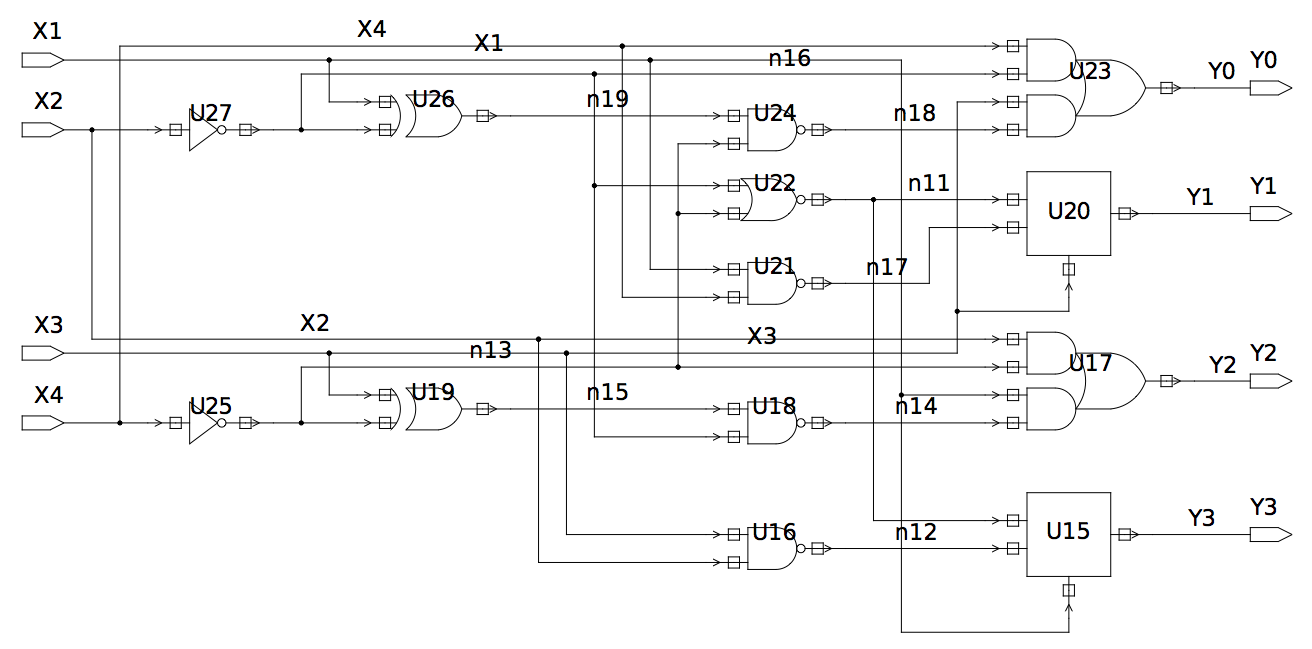
\includegraphics[scale=0.3]{./chapter_optimize/inverse22.png}
    \label{fig:gf4BestInversea}
}
\subfigure[Inversion circuit corresponding to case 20 in Table \ref{tab:inverseCircuitMinimized}]{
    % \rule{2cm}{3cm}
    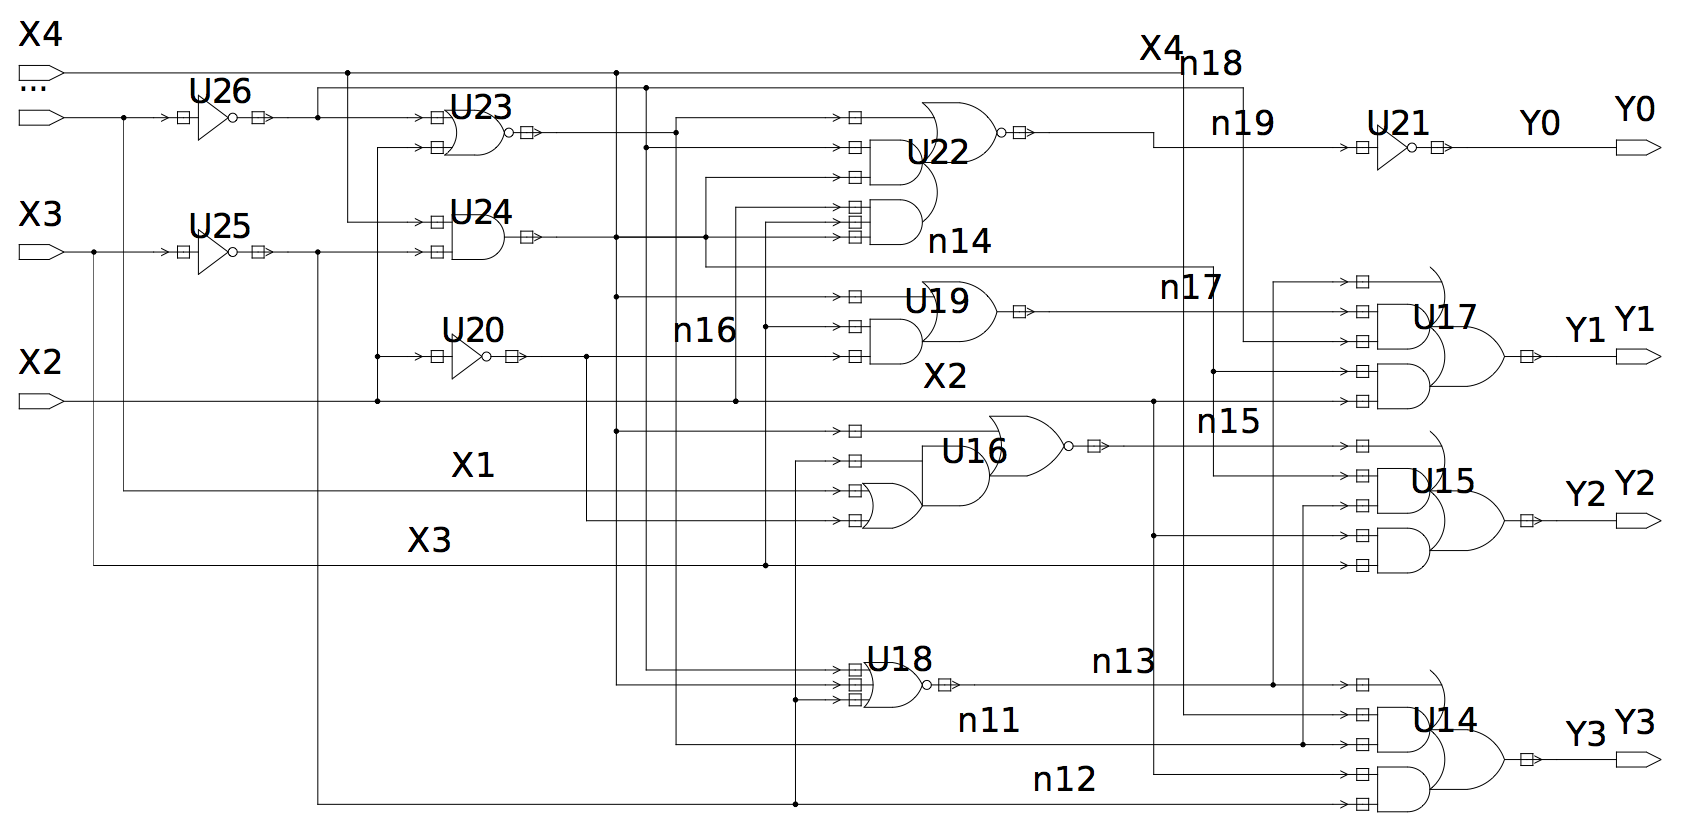
\includegraphics[scale=0.25]{./chapter_optimize/inverse4.png}
    \label{fig:gf4BestInverseb}
}
\caption{RTL schematics for the smallest $GF((2^2)^2)$ and $GF(2^4)$ inversion circuits generated with the Synopsys tool.}
\end{figure}

% However, we have started collaborating with Peralta to explore such modifications in the future as part of the Circuit Minimization Team \cite{CMT}. 

\begin{table} 
\begin{center}
\scriptsize
	\caption{Hardware area requirements for a variety of inversion circuits for fields isomorphic to $GF(2^4)$. The Sum of Products (SOP) entries are unoptimized circuits derived directly from the corresponding truth table, and the optimized entries are those minimized using our modified version of the Boyar-Peralta technique.}
	\label{tab:inverseCircuitMinimized}
	\begin{tabular}{| c | c | c | c | c | c | } \hline  
	\emph{Case} & \emph{Field} & $q(w)$ & \emph{Bases} & \emph{SOP (GEs)} & \emph{Ad-Hoc Optimization (GEs)} \\ \hline
	1 & $GF((2^2)^2)$ & $w^2 + w + v$ & $[1, V]$ and $[1, W]$         & 26.00 & 51.5      \\
	2 & $GF((2^2)^2)$ & $w^2 + w + v$ & $[1, V^2]$ and $[1, W]$       & 27.25 & 49.75     \\
	3 & $GF((2^2)^2)$ & $w^2 + w + v$ & $[V, V^2]$ and $[1, W]$       & 31.50 & 44.0      \\
	4 & $GF((2^2)^2)$ & $w^2 + w + v$ & $[1, V]$ and $[1, W^4]$       & 26.00 & 51.5      \\
	5 & $GF((2^2)^2)$ & $w^2 + w + v$ & $[1, V^2]$ and $[1, W^4]$     & 27.25 & 49.75     \\
	6 & $GF((2^2)^2)$ & $w^2 + w + v$ & $[V, V^2]$ and $[1, W^4]$     & 31.50 & 44.0      \\
	7 & $GF((2^2)^2)$ & $w^2 + w + v$ & $[1, V]$ and $[W, W^4]$       & 22.75 & 36.75     \\
	8 & $GF((2^2)^2)$ & $w^2 + w + v$ & $[1, V^2]$ and $[W, W^4]$     & 20.50 & 22.25     \\
	9 & $GF((2^2)^2)$ & $w^2 + w + v$ & $[V, V^2]$ and $[W, W^4]$     & 27.75 & 37.5      \\
	10 & $GF((2^2)^2)$ & $w^2 + w + v^2$ & $[1, V]$ and $[1, W]$       & 27.25 & 49.75     \\
	11 & $GF((2^2)^2)$ & $w^2 + w + v^2$ & $[1, V^2]$ and $[1, W]$     & 26.00 & 51.5      \\
	12 & $GF((2^2)^2)$ & $w^2 + w + v^2$ & $[V, V^2]$ and $[1, W]$     & 29.00 & 41.75     \\
	13 & $GF((2^2)^2)$ & $w^2 + w + v^2$ & $[1, V]$ and $[1, W^4]$     & 27.25 & 49.75     \\
	14 & $GF((2^2)^2)$ & $w^2 + w + v^2$ & $[1, V^2]$ and $[1, W^4]$   & 26.00 & 51.5      \\
	15 & $GF((2^2)^2)$ & $w^2 + w + v^2$ & $[V, V^2]$ and $[1, W^4]$   & 29.00 & 41.75     \\
	16 & $GF((2^2)^2)$ & $w^2 + w + v^2$ & $[1, V]$ and $[W, W^4]$     & 20.50 & 22.25     \\
	17 & $GF((2^2)^2)$ & $w^2 + w + v^2$ & $[1, V^2]$ and $[W, W^4]$   & 22.75 & 36.75     \\
	18 & $GF((2^2)^2)$ & $w^2 + w + v^2$ & $[V, V^2]$ and $[W, W^4]$   & 29.25 & 34.75     \\
	19 & $GF(2^4)$ & $w^4 + w + 1$ & $[1, W, W^2, W^3]$                & 36.50 & NA  \\
	20 & $GF(2^4)$ & $w^4 + w^3 + 1$  & $[1, W, W^2, W^3]$             & 22.00 & NA  \\
	21 & $GF(2^4)$ & $w^4 + w^3 + w^2 + w + 1$  & $[1, W, W^2, W^3]$   & 26.00 & NA  \\ \hline
	
	% $GF(2^4)$ & $w^4 + w + 1$  & $[w^8, w^4, w^2, w]$             & RUNNING! & RUNNING! & RUNNING! \\
	% $GF(2^4)$ & $w^4 + w^3 + 1$  & $[w^8, w^4, w^2, w]$           & RUNNING! & RUNNING! & RUNNING! \\
	% $GF(2^4)$ & $w^4 + w^3 + w^2 + w + 1$ & $[w^8, w^4, w^2, w]$  & RUNNING! & RUNNING! & RUNNING! \\ \hline
	\end{tabular}
\end{center}
\end{table}
